% !TeX encoding = utf8
% !TeX spellcheck = en

\chapter{Glide Computer}\label{cha:glide}
This chapter focuses on how XCSoar's glide computer works and is
recommended reading so you understand the specific details of
calculations being performed and how to use the software properly.  It
assumes a basic knowledge of cross-country soaring, but is suitable
reading for competition pilots as well as pilots engaging in casual
cross-country touring.


\section{Flight modes}\label{sec:flightmodes}

In order to reduce the pilot's workload, XCSoar is enabled to do 
different things depending on the actual flight's state. XCSoar can 
do this without in-flight interaction of the pilot. The differences are 
reflected by different displays, calculations, and flight information 
amongst others. The four states used by XCSoar are called 
\emph{flight modes}, which are
\begin{itemize}
\item Cruise mode
\item Circling mode
\item Final glide mode
\item Abort mode
\end{itemize}
XCSoar automatically detects the difference between circling flight and 
cruising flight. Circling is enabled when the glider turns (typically 
three quarters of a turn). After about 30~seconds of straight line flight 
the software will switch from circling to cruise mode. Hence, the switch 
is based on a simple condition.

It is also possible to have circling mode switched based on an external 
input (e.g.\ from a pilot-operated switch).

Final glide becomes active when the glider is above final glide 
path with respect to the given navigational task and safety margins. 
The required altitude depends most 
importantly on the adjusted MC value, but also the ground clearance 
is considered. On entering a thermal while in final glide mode for 
gaining some extra safety margin XCSoar will switch to the circling 
mode and back to the final glide mode, once the thermal is left again 
and the final glide condition is still met (i.e.\ the glider is still
above the final glide path, considering MC setting and terrain).

As an example, a powerful feature to be driven by flight modes is the 
switch between different MacCready settings strategies. If you decided
to let XCSoar manage the setting automatically it will maintain a value 
based on past thermals worked out successfully until final glide. 
Instantly MacCready is set to achieve minimal arrival time or what you
set up for final glide (see Section~\ref{sec:auto-maccready}).
\config{final-glide} Hence the switch to final glide mode is based on 
a set of sophisticated computed tactical conditions.

You might force XCSoar to enter final glide mode by skipping all 
remaining turnpoints, if for example conditions get worse and you 
decided to just go home.

Abort mode is invoked manually to give you full control in case of 
emergency via menu.  No automatics --- you decide.  The abort mode
might be understood technically as a special final glide mode with 
concurrent support for multiple optional targets. However, in 
practice the abort mode simply supports your urgent decision where
and how to go finally (see Section~\ref{sec:taskabort}).  In this case,
a safety MacCready value is set. \config{safetyMC} Hence the switch to
abort mode is based on the pilot's cognition.

Due to the fact that the different flight modes typically are reflected in 
differing things being displayed, the frequent XCSoar user might get
used to some kind of watching a `display mode'. This is just the 
default \emph{perceived} after having installed XCSoar without having 
done some advanced configuration. As holds true for almost everything 
within XCSoar, the display's behavior might be changed, adding value 
for the advanced user. But altering things in XCSoar does not influence 
the conditions for entering a flight mode, they do not change.

In order to take full advantage of the flight modes concept, XCSoar 
will \emph{always} show you, which mode is active. A small symbol is 
drawn on the lower right corner of the map area to indicate which flight 
mode the computer is in:

\begin{tabular}{c c c c}%{c c c c}

\includegraphics[angle=0,width=0.75cm,keepaspectratio='true']{icons/mode_cruise.pdf} &

\includegraphics[angle=0,width=0.75cm,keepaspectratio='true']{icons/mode_climb.pdf} &

\includegraphics[angle=0,width=0.75cm,keepaspectratio='true']{icons/mode_finalglide.pdf} &

\includegraphics[angle=0,width=0.75cm,keepaspectratio='true']{icons/mode_abort.pdf}\\
(a) & (b) & (c) & (d)
\end{tabular}

\begin{description}
\item[Cruise (a)]   The glider is not circling and there is either no 
task active, or the task waypoint is not the finish point.
\item[Circling (b)]  The glider is circling (though it may not be climbing).
\item[Final glide (c)]  The glider is not circling and the active waypoint 
is the final one in the task.
\item[Abort (d)]  This manually-triggered mode indicates the immediate 
landing options to the user. (See Section~\ref{sec:taskabort})
\end{description}

The concept of different flight modes enables much more to be automated:
\begin{itemize}
\item \config{screenpages} The InfoBoxes may be set up differently for 
each flight mode. (See Section~\ref{sec:infoboxandpages})
\item \config{circlingzoom} Change zoom level between circling and other 
flight modes (this is called `circling zoom', see Section~\ref{sec:zooming}).
\item \config{variogauge} Switch the vario gauge's reading between Vario 
(gross climb rate) whilst thermalling and airmass lift around you (net) whilst cruising 
(see Section~\ref{sec:variometer}).
\item \config{thermalassistant} When in circling mode, invoke the 
`thermal assistant', a small polar diagram depicting the updraft over 
circular course (see Section~\ref{sec:thermal-assistant}).
\item \config{traildrift} Switch to a so-called drift compensation, 
drawing a wind-compensated trail of the circles you fly to better depict 
wind shear (see Section~\ref{sec:trail}).
\end{itemize}

Take notice, that this list is just an excerpt from an entirety of 
switchable items. You will find numerous dependencies conducted by the 
actual flight mode, whilst further reading this manual. Please pay 
attention to it, because the flight mode concept is one of XCSoar's
fundamental basics. Another very basic scheme deals with how to structure 
information to be displayed together. This information is grouped in
\emph{screen pages}. Further details are given in Section~\ref{sec:infoboxandpages}
``Infoboxes and screen pages''.\config{screenpages}


\section{MacCready setting}

The MacCready setting may be adjusted several ways:
\begin{itemize}
\item For touchscreen/mouse devices, select the MacCready InfoBox field, then
  use the up and down arrow keys.
\item When connected to a supported intelligent variometer, adjusting
  the MacCready setting on the variometer will change the setting
  in XCSoar according to the devices synchronisation configuration (see 
  Section~\ref{conf:comdevices})
\end{itemize}
In addition, an automatic MacCready mode is available as described in
Section~\ref{sec:auto-maccready}.


\section{Glide polar}\label{sec:glidepolar}

The glide polar specifications of a wide selection of glider types,
representing major classes of gliders, are built into XCSoar.
\menulabelr{\bmenug{Config 2/3}\blink\bmenug{Plane}}
If your glider type is not listed, these may be used as an approximation
if no better glide polar can be found.  \config{polar} However, for most 
accurate results, it is advisable to use the correct glide polar for your particular
aircraft type. 
Besides the aircraft type, the correct overall mass of the glider is important for
accurate results. 
The preflight check of your tactical glide computer certainly 
includes a check of the correct settings for water ballast, with regard to the 
configured dry mass. Because XCSoar does not offer a setting for the pilots 
weight you are free to include the latter to the dry mass setting, or the 
water ballast setting.

On top of the polar and mass configuration the glide polar is adjustable 
in flight to take into account performance degradation due to bugs or 
rain droplets.

The build-up of bugs on the wing's leading edge, as well as rain
droplets on the wing, affect the aerodynamic performance.  It is the
pilot's responsibility to judge and update the bugs value during
flight.  The bugs value is expressed as a percentage of degradation 
compared to the clean glider's performance.
For example, at 0\% bugs value, the glider
performs as a clean glider, and at 50\% bugs value, the glider's
sink rate is doubled when compared to a clean glider. The calculation 
scales linearly in-between. 

\menulabel{\bmenug{Info 1}\blink\bmenug{Analysis}}
\begin{center}
\includegraphics[angle=0,width=\linewidth,keepaspectratio='true']{figures/cut-clean-dirty-polar.png}
\end{center}
Knowing all this, a meaningful setting for a worst-case bug polluted wing could
scale down the polar by 30\%. Some experimentation may be required to determine 
appropriate settings for bugs, because the performance degradation experienced 
by different glider types may be different.

Alternatively, you can enable the ``Auto bugs'' feature which adds 1\% to the
bugs setting after each full hour of flying.   This feature is set via

\button{Config 1}\blink\button{System}\blink\button{Glide Computer}\blink\button{Safety Factors}\blink\button{Auto bugs}

The ballast is set in litres of water. 
Depending on the specifically set dry mass of the glider, this may optionally 
include a weight margin to provide for different pilot weights.
  When flying with no ballast, a heavy pilot
may set a ballast value of perhaps 15~l so that the polar is
appropriately adjusted for the increased cockpit weight.

\begin{center}
\menulabel{\bmenug{Info 1}\blink\bmenug{Analysis}}
\includegraphics[angle=0,width=\linewidth,keepaspectratio='true']{figures/overlay-non-balasted-polar.png}
\end{center}


\section{Flight setup dialogue}\label{sec:flight-setup}
Use the flight settings dialogue to modify the all up weight of the glider both
before and during flight, as well as to set the QNH pressure.  

\menulabel{\bmenug{Config 1}\blink\bmenug{Flight}}
\begin{center}
\includegraphics[angle=0,width=0.45\linewidth,keepaspectratio='true']{figures/dialog-basicsettings.png}
\end{center}

The `bugs' setting determines the amount the polar is degraded
due to contamination during a long flight.  A `bugs' setting of 0\%
will cause the software to use the clean polar. A `bugs' setting of
50\% will degrade the polar and effectively double the sink
rate for a given airspeed.

The ballast setting is used to modify the polar to account for any
water ballast carried during the flight. Ballast is shown in litres,
and should be set to correspond to the correct water ballast added
before flight.  The ballast setting modifies the polar to account for
the indicated load of water ballast.

Use this dialogue both before and during the flight to record the mean
sea level atmospheric pressure, also known as QNH pressure.  The
software uses the values entered to convert airspace flight levels
into altitudes.  If connected to a supported intelligent variometer
with an altimeter, the altitude is updated on this dialogue as the QNH
pressure is adjusted.  This makes it easy to set the QNH pressure if
the airfield elevation is known.

The maximum forecast ground temperature is used by the convection
forecast algorithm (see Section~\ref{sec:convection-forecast}) in its
determination of estimated convection height and cloud base.

\tip{} It is possible to configure XCSoar to display the basic
settings dialogue when it starts up.

On system startup, after the GPS has acquired lock, and if a
barometric altitude source is connected (e.g.\ Vega, AltairPro,
FLARM), the QNH is automatically adjusted.  This adjustment sets the
QNH such that the barometric altitude equals the terrain altitude.

The QNH is only updated if the aircraft is on the ground for more than
10~seconds, so that if XCSoar is restarted during flight, QNH will not
be adjusted.  The update also only occurs if the terrain database is
valid at the current aircraft location.

\section{Speed command display}

When used in conjunction with an intelligent variometer that produces
indicated airspeed measurements, a speed command chevron is drawn
on the right side of the map display.  If the glider is flying slower
than the optimal speed, the chevrons are red and point downwards.  If
the glider is flying faster than the optimal speed, the chevrons are
green and point upwards.  If the speed is approximately optimal, no
chevrons are drawn.

%{\it DIAGRAM SHOWING SPEED COMMAND CHEVRONS}

Depending on the configuration, speed command chevrons can be
displayed on the right side of the map area, or on the variometer
gauge.


\section{Speed to fly}\label{sec:stf}

XCSoar continuously calculates two types of speed to fly:
\begin{description}
\item[MacCready speed]  This is the best speed to fly during cruise
  in still air, adjusted for wind if in final glide mode.
\item[Dolphin speed]  This is the instantaneous, best speed to fly
  in rising or descending air, adjusted for wind if in final glide
  mode.
\end{description}  

The user can specify a maximum maneuvering speed in the configuration
settings, which limits the speed-to-fly in MacCready calculations to
realistic values.

Different pilots have personal preferences as to whether they prefer
to fly in so-called `block MacCready' style, in which they fly
constant speed between thermals according to the MacCready speed; or
to fly in `dolphin' style, in which they fly at varying speeds
according to the continuously changing Dolphin speed value.

\begin{maxipage}
\begin{center}
\includegraphics[angle=0,width=0.8\linewidth,keepaspectratio='true']{figures/figure_speed_to_fly.pdf}
\end{center}
\end{maxipage}

A configuration option `Block speed to fly' (see
Section~\ref{sec:final-glide}) can be used to specify whether dolphin
or block speed to fly is used.  The infobox `V Opt' shows the optimum
speed according to whichever mode is selected.  When connected to the
Vega intelligent variometer, the speed command sounds are based on
this optimum speed value.


\section{Speed to fly with risk}\label{sec:safety-factor}

  The speed to fly system can be compensated for risk, in which the
  MacCready setting used for calculating the speed to fly (in both
  Block or Dolphin modes) is reduced as the glider gets low.

  Many pilots typically wind down the MC as they get low --- this
  feature performs this automatically.  The theory governing how this
  is implemented in XCSoar is based loosely on the paper by John
  Cochrane, ``MacCready Theory with Uncertain Lift and Limited
  Altitude'', \emph{Technical Soaring}, 23 (3) (July 1999) 88--96.

\url{https://www.johnhcochrane.com/s/newmcred.pdf}

  A configuration parameter $\gamma$ (`STF risk factor', in the
  configuration settings under page `Glide Computer') controls how the
  risk MC value is calculated.  The $\gamma$ factor determines the
  fraction of the current MacCready setting as a function of the
  height fraction.  The height fraction used in this calculation is
  the ratio of the height above terrain ($h$) to the height of the
  maximum climb above the
  terrain ($h_{top}$, this will usually be close to cloudbase).
  The $\gamma$ setting thus represents the
  fraction of the total available climb (cloudbase minus terrain) at
  which you would wish to abandon the task and begin to prepare for a
  landout.  Thus, low $\gamma$ values indicate a higher tolerance for
  landout risk than higher values of $\gamma$.

  For the default value, $\gamma=0.0$, there is no compensation ---
  the risk MC is the same as the MC setting.  For $\gamma=1.0$, the
  risk MC is scaled linearly with the height fraction $h/h_{top}$.
  For intermediate values of $\gamma$, the risk MC varies smoothly
  with the height fraction, such that the risk MC is small only when
  low.

  Low values of $\gamma$ are best when pilots do not want to slow down
  as they get low (but risk out-landing); high values of $\gamma$ can
  be used for very cautious pilots but will result in lower average
  speeds.

  A value of $\gamma=0.3$ is recommended.

\begin{center}
\includegraphics[angle=0,width=\linewidth,keepaspectratio='true']{figures/riskmc.png}
\end{center}


\section{Safety heights}\label{sec:safety-heights}

Three safety heights are defined to provide a degree of safety margin
in glide computer calculations.  

The safety heights are:
\begin{description}
\item[Arrival height (a)]  This is the elevation above ground at which
 the glider is required to arrive at least.
 Typically, you want to include height for a safe landing circuit, plus
 some safety margin for hazardous vertical/horizontal air movements and
 resulting errors of computed route and speed.
 This value is used in final glide calculations as
 well as the determination and display of reachable landable fields.
\item[Terrain clearance (b)]
 This is the elevation above ground, below which any computed glide
 path is considered to provide inadequate clearance to the terrain.
 The terrain clearance value affects the glide range display, and if
 the final glide at any point dips below the terrain clearance
 elevation above ground, a warning marker (large red cross) is drawn
 on the screen.  If the terrain elevation model is invalid or out of
 range, then the glide range display and the terrain warning marker is
 disabled.
\item[Break-off height (c)]  This is the elevation above ground, below which 
 it is recommended for pilots to consider the cross-country task
 failed and to concentrate on finding a suitable field to land in.
 Currently, this break-off height does not affect XCSoar in any way but
 it is referenced in the manual.
\end{description}

\begin{maxipage}
\begin{center}
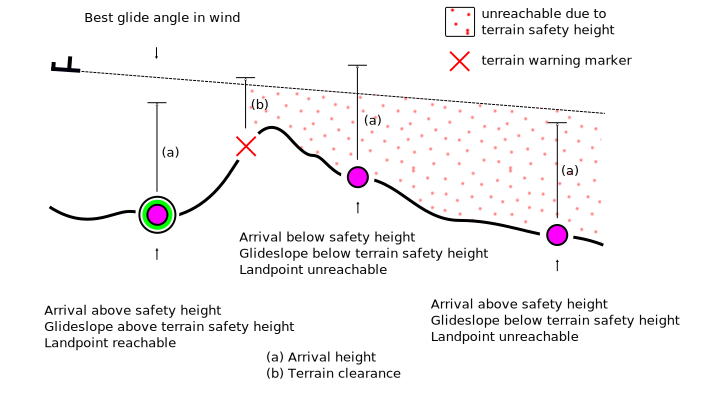
\includegraphics[angle=0,width=\linewidth,keepaspectratio='true']{figures/figure_terrain.pdf}
\end{center}
\end{maxipage}

\warning{}
These may be set to zero but this is highly discouraged since all
glide computers, instruments and data sources (such as terrain
elevation models) are subject to some degree of error and the
atmosphere through which the glider flies is also unpredictable.

XCSoar determines the elevation above sea level of any turn point or
landing point either from the waypoint file, or if no height is
specified in the waypoint file, from the terrain file.

\textbf{The estimated arrival altitude displayed next to landable
  waypoints is by default calculated for best glide angle at zero
  MacCready ring setting (MC$=0$), adjusted for wind.  However, a
  safety MacCready setting may be configured to modify the MacCready
  setting used in this calculation, as described below.}

Landable fields are only marked as reachable if the estimated arrival
elevation above ground is above the arrival altitude safety height,
and the glide path does not intersect the terrain clearance safety
elevation.

At all times, if the final glide through terrain marker (a red
cross) is displayed on the screen, then the glider must climb in order
to safely reach the destination.

When calculating the arrival heights of landable fields (for map
display purposes and in abort mode), a safety MacCready value can be
specified in the configuration settings.  This safety value is set to
zero by default.  Larger values make the arrival height calculation
more conservative.


\section{Final glide calculator}

The final glide calculator uses many sources of information when
determining the altitude required to reach your goal or the next
waypoint. These are:

\begin{itemize}
\item The glider's polar data;
\item The wind speed and direction;
\item The distance and bearing of the goal or waypoint;
\item The MacCready setting;
\item The altitude of the waypoint or goal;
\item A user specified safety margin (arrival height and terrain clearance).
\item The glider's total energy if XCSoar is connected to
  an instrument with an air speed indicator.
\end{itemize}

From the parameters shown above, two altitudes are derived.
\begin{description}
\item[Altitude required]
This calculation is the total altitude required for the glider to
reach the goal plus any user safety margin. 
\item[Altitude difference]
This calculation is the altitude required to glide to the goal plus
any safety arrival altitude plus the altitude of the goal, minus the
altitude above mean sea level of the glider.  The result represents
either your height above glide slope, or your arrival height at goal.
If no goal altitude is provided in the turn-point file, XCSoar will use
the terrain file altitude at the goal.
\end{description}

The final glide calculation is extended to calculate the altitudes
required and difference to complete the entire task.  This capability
is sometimes referred to as final glide around multiple turn points.
The altitude difference to complete the task is displayed continuously
as an arrow and in numeric form on the left-hand side of the map area
of the screen.

The altitude required is adjusted for energy, compensating for
the fact that the kinetic energy of the glider can be converted to
height (potential energy).  The kinetic energy that is convertible to
height is calculated from the difference in the true airspeed to the
true airspeed for best glide.  This compensation is most accurate when
airspeed data is available to XCSoar, otherwise the true airspeed is
estimated from the wind speed and ground speed.


\section{Display of required altitude difference}

On the left side of the map display, a box displays the calculated
altitude difference required for the glider to complete the task, or
reach the final waypoint.  If the glider is above the minimum altitude
required, a green arrow bar is drawn above the box indicating the
amount of excess height.

If the glider is below the minimum altitude required, a red arrow bar is
drawn below the box indicating the amount of height deficit.  If,
however, there are landable waypoints within glide range, but the
glider is below the minimum altitude required to complete the task, the
bar is coloured amber.

\begin{center}
\begin{tabular}{c c}
\emph{Above} & \emph{Below} \\
\includegraphics[angle=0,keepaspectratio='true']{figures/cut-fg-above.png} &
\includegraphics[angle=0,keepaspectratio='true']{figures/cut-fg-below.png} \\
\multicolumn{2}{l}{The scale of the final glide bar is $+/-$ 500~meters.} \\
\multicolumn{2}{l}{A bar beyond this scale is indicated by a chopped-off tip.}
\end{tabular}
\end{center}
\tip{}
At this point it must also be mentioned, that the indicated height below the glide
path is not just a plain difference of glide path and current altitude. Depending 
on the setting `predict wind drift' (On) the `Below' indicator 
shows the required height to gain by thermalling. \config{predict-drift}
The required height might be quite a bit more with headwind, as well as a bit less
with tailwind. 
Otherwise (`predict wind drift' set to Off), it is just the plain
altitude difference.



\subsection*{Dual altitude required bars}

The final glide bar has been extended to show the effect of MacCready
setting on the altitude difference to complete the task.  The display
shows with a brighter split arrow the \emph{altitude difference calculated at zero
MacCready}, as well as the usual arrow that displays the
altitude difference calculated at the current MacCready setting.

The number shown in the box next to the final glide bar still shows
the altitude difference at the current MacCready setting.

Examples of the appearance in various configurations with the additional \emph{MC$=0$} 
bar display is shown below:

\begin{description}
\item[Above final glide] (current MC$=0.7$)
\smallsketch{figures/fig-finalglide-allabove.png}
  Here the display shows that at the current MacCready setting, the aircraft
  is above final glide (filled arrow).  The split arrow shows the additional
  excess height.

\item[Below/above final glide] (e.g. MC$=1.8$)
  Here the display shows that at the current MacCready setting, the aircraft
  is below final glide (filled amber arrow).  The split green arrow
  shows that at MC$=0$, the aircraft is above final glide.

\smallsketch{figures/fig-finalglide-halfabove.png}
  In this situation, if the glider is climbing, the pilot can assess
  whether to leave the thermal early and commence a final glide
  descent at a reduced MacCready setting; or continue to climb.  It is
  useful to switch on the auto MacCready setting as this will
  automatically adjust the MacCready value to the optimal value ---
  and then it is simple for the pilot to compare the achieved lift
  rate with the MacCready value.  When the achieved lift rate drops
  below the MacCready value, the thermal should be left.

\item[Below final glide] (e.g. MC$=2.5$ and with less height)
\smallsketch{figures/fig-finalglide-littlebelow.png}
  Here the display shows that at the current MacCready setting, the aircraft
  is below final glide (filled red arrow).  The tip of the red arrow is chopped off
  to show that the altitude undercut the 500~meter limit the arrow can scale on.
  The split slightly brighter red arrow shows that by reducing the MacCready 
  setting to zero, the aircraft still is far from final glide.

\item[Below final glide] 
  Here the display shows that at the current MacCready setting, the aircraft
  is below final glide (red arrow).  The split brighter red arrow
\smallsketch{figures/fig-finalglide-allbelow.png}
  shows that even at MC$=0$ the aircraft is well below final glide.
\end{description}


\section{Task speed estimation}\label{sec:task-speed-estim}

Some of XCSoar's internal calculations make use of estimates of the
time required to reach each waypoint in the task.  This information is
used in some {\InfoBox} displays, Assigned Area Task calculations, and
sunset warnings.

The glide computer assumes the glider's average cross-country speed is
equal to that achievable under classic MacCready theory taking wind
into account, with the current MacCready setting.  This method is used
for estimating arrival times and task finish time.

The following task speed measures are defined:
\begin{description}
\item[Task speed achieved]  This is the task speed to date, compensated
for altitude differences from the task start altitude.
\item[Task speed average]  This is the task speed to date compensated
for altitude required to complete the task.
\item[Task speed remaining]  This is the task speed estimated for the
  remainder of the task according to MacCready theory.
\item[Task speed estimated]  This is the task speed estimated for the entire 
task, start to finish, assuming flying the remainder of the task according 
to MacCready theory.
\item[Task speed instantaneous]  This is the instantaneous estimated speed 
along the task.  When climbing at a rate equal to the MacCready setting, this 
number will be similar to \emph{Task speed remaining}.  When climbing more slowly 
than this or cruising in a direction other than directly toward the active 
waypoint, this number will be lower than \emph{Task speed remaining}.  In cruise 
at the optimum speed directly toward the active waypoint in air that has no 
vertical motion, this number will be similar to \emph{Task speed remaining}.

This measure, available as an {\InfoBox}, is useful as a continuous
indicator of cross-country performance.  It is not used in any
internal calculations.
\end{description}

\tip{}For an assigned area task (AAT), the positions of any remaining targets 
with the \emph{Optimized} box checked are automatically adjusted (if room for 
such adjustment is available) to give an estimated total task time of five 
minutes more than the task's \emph{AAT min. time}.

Also, a measure called \emph{Achieved MacCready} is calculated.
This is computed by finding the MacCready setting that under classical
MacCready flight would produce the same task speed as has been
achieved so far.  This value is higher than the actual MacCready setting when
the glider has climbed faster than the actual MacCready setting or when the
glider has flown in cloud streets, for example.  \emph{Achieved MacCready} is 
shown in the \emph{Status} dialogue's \emph{Task} tab but is not available as 
an InfoBox.

An "achieved" task speed includes compensation for the glider's net change in 
altitude so far.  For example, two gliders flying the same task can have
different "achieved" task speeds even if they have both flown the exact same
distance in the exact same amount of time.  The higher-altitude glider will
have a greater "achieved" task speed.  In fact, a glider that has flown 
\emph{less} distance in the same amount of time could have a greater 
"achieved" task speed if its altitude is enough higher than that of the
farther-ahead glider.

While flying an AAT, task speed measures may change relatively quickly when 
the glider is inside a turn area or when AAT range or target location is
adjusted by the pilot.  This is due to changes in \emph{task distance 
achieved} and \emph{task distance remaining} when such events occur.


\section{Optimal cruise track}

In order to help reduce the cross-track error when flying between
non-final waypoints, XCSoar calculates an adjustment to the cruise
track, called the `optimal cruise track'.  This track is adjusted so
that it compensates for the wind drift incurred when circling, and as
such it needs to estimate the proportion of time spent circling
according to classical MacCready theory.

\begin{center}
\begin{maxipage}
\centering
\def\svgwidth{0.8\linewidth}
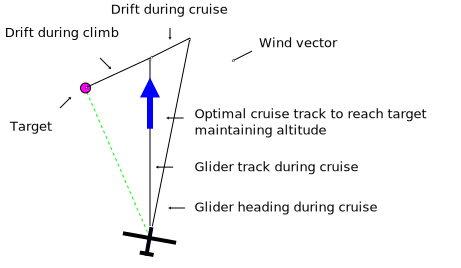
\includegraphics[angle=0,width=0.8\linewidth,keepaspectratio='true']{figures/figure_optimal_cruise.pdf}
\end{maxipage}
\end{center}

The optimal cruise track is displayed on the map area as a large blue
arrow, and it recommends the glider steers so that the glider's track
is lined up with the blue arrow during cruise.  For example, if the
display is oriented `Track-Up', then steer so the blue arrow points
directly up.

The glide computer accounts for wind drift during circling to provide
an `optimal cruise track' vector, which indicates the track the glider
should follow during cruise such that it will arrive at the waypoint
in minimum time.  This vector is displayed on the map as a blue arrow.
When the wind is negligible, or when the computer is in final glide
mode, this arrow will point along the black line that indicates the
track to the next waypoint.

The calculation and display of optimal cruise track is a unique
feature of XCSoar.  Commonly, when cruising between thermals, glide
navigation systems direct the glider to steer so that the glider's
track points directly at the target.  Ideally, the glider's track is
collinear with the line from the previous to next waypoint, such that
the cross-track error is small and hence the glider travels the
minimum distance between waypoints.

However, because the glider usually has to stop cruising in order to
climb in lift, whilst circling the glider drifts downwind and
therefore the cross track error can increase.  After several cycles of
cruise-climb, the overall track becomes curved.
%
%{\it DIAGRAM SHOWING CRUISE TRACK NOT ADJUSTED FOR WIND}

For the case where the final waypoint is active and one is above final
glide, circling is not necessary so this simple scheme is optimal.


\section{Auto MacCready}\label{sec:auto-maccready}

XCSoar can adjust the MacCready ring setting automatically to relieve the
workload on the pilot.  Two methods of updating the MacCready ring setting
are available:
\begin{description}
\item[Final glide]  During final glide, MacCready is adjusted in order to
 arrive at the finishing point in minimum time.  For OLC Sprint tasks,
 the MacCready is adjusted in order to cover the greatest distance in the remaining
 time and reach the finish height.
\item[Trending average climb] When not in final glide, MacCready is adjusted
to the trending average climb rate based on all thermals.
\end{description}
Additionally, both methods may be used, so that before reaching final glide,
the MacCready setting is adjusted to the average climb rate, and during final
glide it adjusts the setting to give minimum time to arrival.

The method that is used is defined in the configuration settings dialogue as the
field ``Auto MC Mode''.  The default setting is ``Both''.

When Auto MacCready is enabled, the MacCready infobox displays `MC auto'
instead of `MC manual'; and the MacCready indicator in the variometer
gauge displays `AutoMC' instead of `MC'.
To benefit the most from the automatic MC adjustment XCSoar propagates the MC
value to the connected intelligent variometer (if it supports).

The Auto MacCready methods are described in further detail below.


\subsection*{Final glide}

When above final glide altitude, the MacCready ring setting may be
increased, resulting in a higher speed to be commanded.  Because the
ring setting has increased, this also increases the minimum strength
of the thermal that would be efficient to stop and circle in.

Similarly, when below final glide altitude, the MacCready ring setting
may be decreased, resulting in a lower speed to be commanded.  Because
the ring setting has decreased, the pilot may be prepared to stop and
circle in weaker thermals.

Auto MacCready performs this adjustment automatically and
continuously.  Typically, it is meaningless to enable this mode before
reaching final glide altitude, or nearly so, because early in the
flight the glider will be very much below the final glide altitude and
the Auto MacCready function would then drive the MacCready ring
setting to zero.

\begin{maxipage}
\begin{center}
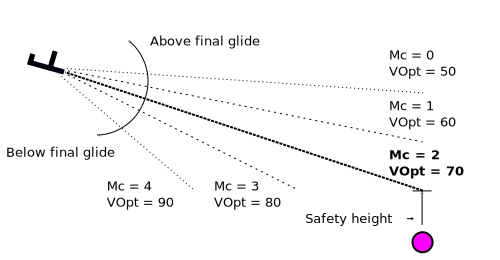
\includegraphics[angle=0,width=0.8\linewidth,keepaspectratio='true']{figures/figure_auto_maccready.pdf}
\end{center}
\end{maxipage}


\subsection*{Average climb}

This method sets the MacCready to the average climb rate achieved
across all thermals in the current flight.  As such, it takes into
account the time spent centering the thermal.  The value is updated
after leaving a thermal.

Since MacCready theory is optimal if the MacCready setting is the
average climb rate of the next expected climb, this method may give
sub-optimal performance (commanding speed too slow) if the conditions
are improving; and similarly may be non-conservative if the conditions
are deteriorating (commanding speed too high).  Similarly, if the pilot
continues to climb in weak thermals, this will reduce the average
and may therefore encourage the pilot to continue to select weak thermals.

As a result of these limitations, the pilot should be aware of how the
system operates and adjust his decision-making accordingly.


\section{Analysis dialogue}

The analysis dialogue can be used to check the glide polar.  
\menulabel{\bmenug{Info 1}\blink\bmenug{Analysis}}

The polar page shows a graph of the glide polar at the current bugs
and ballast setting.  It also shows the calculated best L/D and the
speed at which it occurs, and the minimum sink and the speed at which
it occurs.  The current aircraft all up weight is displayed in the
title.

\begin{center}
\includegraphics[angle=0,width=0.8\linewidth,keepaspectratio='true']{figures/analysis-glidepolar.png}
\end{center}

In this dialogue page, the `Settings' button opens the flight settings
dialogue (e.g.\ to adjust the bugs/ballast).

The glide polar page of the analysis dialogue shows the average total
energy sink rate at each speed achieved in flight, when connected to a
supported intelligent variometer (e.g.\ Vega).  This facility allows
pilots to perform test flights in stable atmospheric conditions, such
as on calm days with no wind, and inspect the measured glide polar.
By comparing the measured glide polar with the model glide polar, this
enables investigation of whether the glider is being flown optimally
with respect to flap settings and also to investigate the benefits of
performance optimisation such as sealing control surfaces, etc.

Data is collected only when in cruise mode and at G loading between
0.9 and 1.1; so pilots performing test flights should attempt to fly
smoothly with wings level.

\begin{center}
\includegraphics[angle=0,width=0.8\linewidth,keepaspectratio='true']{figures/shot-glidepolar.png}
\end{center}


\section{Flight notifications}

 Notifications, appearing as status messages, appear when the
 following conditions are detected: 
\begin{itemize}
\item Estimated task time too early for
 AAT 
\item Estimated arrival at finish past sunset
\item Significant wind change
\item Transition to above/below final glide
\end{itemize}
% JMW more detail here
